\chapter{Pipeline Evaluation}

This chapter presents the evaluation of the pipeline as a whole system.
First, the used evaluation algorithms are explained, together with the notions of \ac{TP}, \ac{FP} and \ac{FN} in their respective context.
For object detection this has already been explained in section \ref{sec:tpfpfn}.
An overview of this chapter can be found in figure \ref{fig:eval_pipeline_overview}.
At the end of this chapter, the results are presented with a thorough evaluation.

\begin{figure}
\begin{center}
    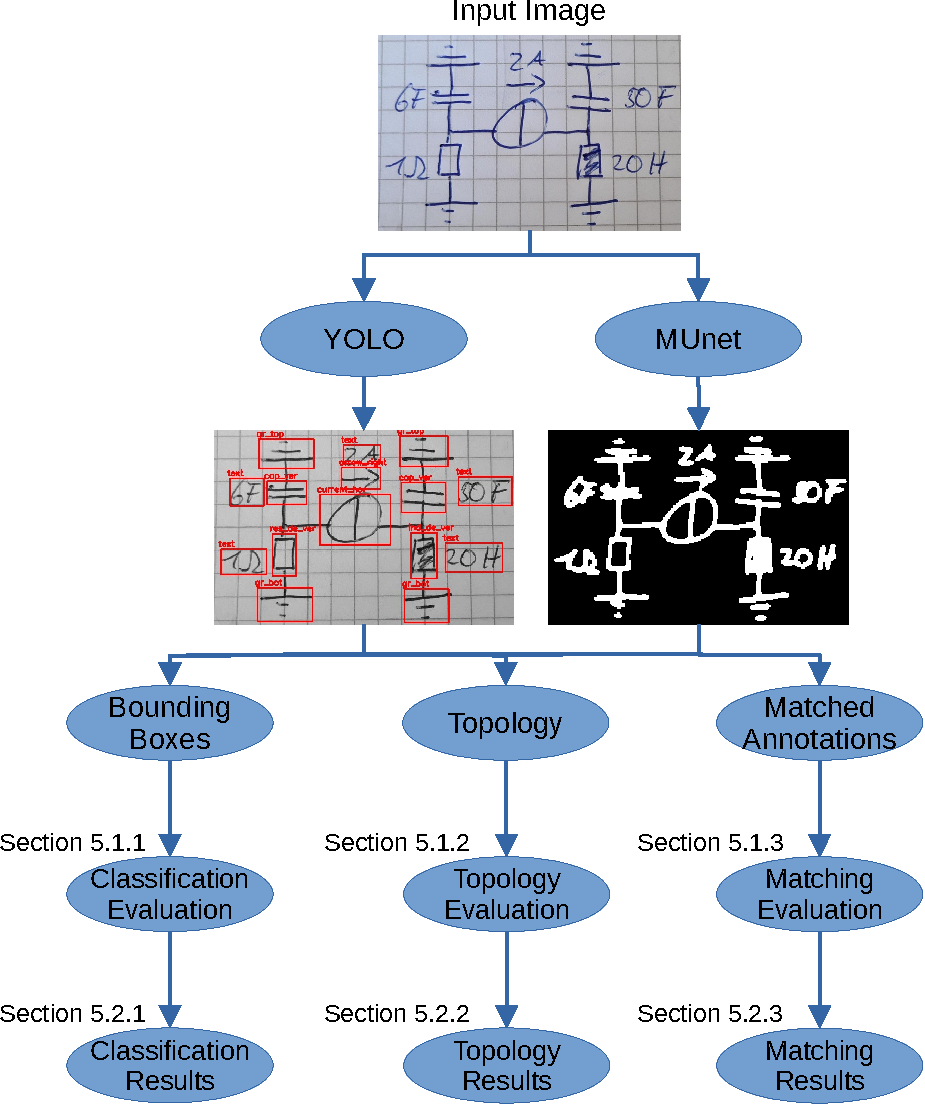
\includegraphics[width=\columnwidth]{imgs/pipeline/eval_pipeline_overview_crop.pdf}
    \caption{Overview of the evaluation pipeline. Evaluation is split into classification evaluation of bounding boxes, topology evaluation and matching evaluation.}
    \label{fig:eval_pipeline_overview}
\end{center}
\end{figure}

\section{Evaluation Algorithm}
\label{sec:eval_algo}

\subsection{Classification}

The evaluation of the \ac{YOLO} network was already done in section \ref{sec:yolo_final} based on the \ac{mAP} metric.
This metric considers multiple \ac{IoU} thresholds in its calculation and provides a general detection performance.
However, in the context of topology generation, a prediction with a bad \ac{IoU} with its ground truth could still lead to a correct prediction of the topology.
Therefore, for the evaluation of the full pipeline the matching of bounding box predictions is done using a fixed \ac{IoU} threshold.
To find an initial guess of the threshold, first the maximum occlusion \ac{IoU} was obtained from the training and validation dataset, by calculating the \ac{IoU} between each ground truth in an image.
The maximum occurring \ac{IoU} was found at 14\%, which means that in general the dataset has low occlusion.
Under the assumption that the size of the predicted bounding boxes will be greater than the size of the respective ground truth bounding boxes the \ac{IoU} was chosen to be bigger than the maximum occlusion \ac{IoU}.
For the evaluation the \ac{IoU} threshold was set to 30\%.
Furthermore, for the evaluation in this section, the predictions are provided with the \acp{TP}, \acp{FP} and \acp{FN} values, as well as with metrics, which can be calculated from those.

The segmentation outcome is not further quantified since a re-quantification would just be a repetition of section \ref{sec:munet_final}, where the final results of the \ac{MUnet} were presented.
However, the outcome of the topology highly depends on the segmentation, hence a bad segmentation will result in a bad topology similarity between ground truth and prediction.

\subsection{Topology}

The similarity of the predicted and the ground truth topology is measured, based on a hypergraph adjacency matrix (section \ref{sec:hypergraph_topology}).
To recall, a hypergraph is defined as: $\mathbf{H} = \{\mathbf{V}, \mathbf{E}\}$, with the vertices $\mathbf{V} = \{v_1,...,v_n\}$ and the hyperedges, $\mathbf{E} = \{\mathbf{e_1},...\mathbf{e_n}\} = \{\{v_i,...,v_j\},...,\{v_x,...,v_y\}\}$.
Further, a subedge and the amount of subedges present in an hyperedge is defined as: $\mathbf{S}(\mathbf{e_i}) = \{ \{v_1,v_2\}\ |\ \{v_1,v_2\} \in \mathbf{e_i},\ \mathbf{e_i} \in \mathbf{E}\}$, $\#\mathbf{S}(\mathbf{e_i}) = \{ \#\mathbf{e_i} - 1\ |\  \mathbf{e_i} \in \mathbf{E}\}$, where \# is the length operator for a set.
For the presented algorithm the notation $TP_h$, $FP_h$ and $FN_h$ is used, where the $*_h$ indicates that those are quantizations related to the hypergraph evaluation.

The presented algorithm is inspired by the graph edit distance algorithm \cite{graph_edit_distance}, which calculates the cost for transforming one graph into another.
However, graph edit distance counts only the needed steps without considering the type of the error.
Therefore, in this work the error type notions are also presented.
The full algorithm is summarized in algorithm \ref{alg:topology_eval}.

\subsubsection{The subedges in prediction and ground truth are the same}
This occurs when the tested ground truth hyperedge $\mathbf{e_i}$ and predicted hyperedge $\mathbf{\hat{e}_i}$ have the same vertices in them.
The amount of $TP_h$ ($\#TP_h$) occurring from a perfect match is defined as:

\begin{equation}
    \#ground\_truths = \#TP_h(\mathbf{e_i}) = \#S(\mathbf{e_i})
    \label{eq:tph}
\end{equation}

% In an error free context (no $\#FN_h$, no $\#FP_h$), $\#TP_h$ is equal to the amount of all possible positive predictions.

\subsubsection{A subedge is missing}
This occurs when a perfect match can not be found directly, but only through recombination of predicted hyperedges.
Consider the following example:

\begin{itemize}
    \item Ground truth $\mathbf{H}$: $\mathbf{V} = \{v_1, v_2, v_3\}$, $\mathbf{E} = \{\{v_1, v_2, v_3\}\}$
    \item Predicted $\mathbf{\hat{H}}$: $\mathbf{\hat{V}} = \{v_1, v_2, v_3\}$, $\mathbf{\hat{E}} = \{\{v_1, v_2\}, \{v_3\}\}$
\end{itemize}

In this example no perfect match can be obtained between the ground truth and the prediction.
However, recombining $\mathbf{\hat{e}_1}$ and $\mathbf{\hat{e}_2}$ would results in $\mathbf{e_1}$, which allows to calculate a perfect match.
Calculating a perfect match with equation \ref{eq:tph} would result in $\#ground\_truths = 2$.
However, the perfect match could only obtained through recombination.
Therefore, there exists a $\#FN_h$, which is defined as:

\begin{equation}
    \#FN_h = \#(recombined\ hyperedges\ for\ perfect\ match) - 1
    \label{eq:fns}
\end{equation}

In this example $\#FN_h = \#(\{\{v_1, v_2\}, \{v_3\}\}) - 1 = 2 - 1 = 1$.
Comparing the notion of ground truth, $TP_h$ and $FN_h$ to object detection, this shows a close relation and the amount of ground truths can be calculated through:

\begin{equation}
    \#ground\_truths = TPs + FNs
    \label{eq:all_possible}
\end{equation}

The same notion applies here.
Therefore, the $\#TP_h$ can be calculated using equation \ref{eq:all_possible}:
$\#TP_h = \#ground\_truths - \#FN_h = 2 - 1 = 1$.

Naturally the equations \ref{eq:fns} and \ref{eq:all_possible} extend to the case, where the hyperedges of $\mathbf{\hat{H}}$ are $\mathbf{\hat{E}} = \{\{v_1\}, \{v_2\}, \{v_3\}\}$.
Again, to have a perfect match all hyperedges have to be recombined, hence: $\#FN_h = \#(\{\{v_1\}, \{v_2\}, \{v_3\}\}) - 1 = 3 - 1 = 2$, $\#ground\_truths = 2$ and therefore $\#TP_h = \#ground\_truths - \#FN_h = 2 - 2 = 0$.

\subsubsection{A subedge too much}
This case occurs, when a perfect match can only be obtained by splitting a predicted hyperedge, due to $\mathbf{e_i} \subset \mathbf{\hat{e}_j}$.
Consider the following example of a ground truth and predicted hypergraph:

\begin{itemize}
    \item Ground truth $\mathbf{H}$: $\mathbf{V} = \{v_1, v_2, v_3, v_4\}$, $\mathbf{E} = \{\{v_1, v_2\}, \{v_3, v_4\}\}$
    \item Predicted $\mathbf{\hat{H}}$: $\mathbf{\hat{V}} = \{v_1, v_2, v_3, v_4\}$, $\mathbf{\hat{E}} = \{\{v_1, v_2, v_3, v_4\}\}$
\end{itemize}

The hyperedge $\mathbf{\hat{e}_1}$ is split into: $\mathbf{Split} = \{\{v_1, v_2\}, \{v_3, v_4\}\}$.
A perfect match can now be obtained from the newly created hyperedges.
The first perfect match is obtained from $\{v_1, v2\}$, with $\#TP_h = 1$ and the second one from the remaining hyperedge $\{v_3, v4\}$ also with $\#TP_h = 1$, therefore $\#TP_h = 1 + 1 = 2$.
However, the perfect matches could only be obtained through splitting, hence additionally $FP_h = 1$, because it required one split to obtain the results.

% The algorithm here then removes the ground truth hyperedge from the predicted hyperedge, by setting all values in the predicted hyperedge to 0.
% The remaining parts of the predicted hyperedge are then again reused for the recombination.

% Therefore, by obtaining the amount of ground truths with equation \ref{eq:tph}, which is the $\#TP_h$ obtained in a perfect match and considering that the perfect match could only be calculated by recombining $\hat{e}_1$ and $\hat{e}_2$ the following can be obtained: $\#(ground\_truths) = 2$, $\#FN_h = 2 - 1 = 1$ and using equation \ref{eq:all_possible} $\#TP_h = \#(ground\_truths) - \#FN_h = 2 - 1 = 1$.

% As mentioned all \ac{TP} calculations are only performed with perfect matches.
% In this case a perfect match can be recreated by combining the two hyperedges in $\hat{H}$.
% The resulting perfect match would have $TPs = 2$, due to the fact that this is the amount of subedges $\#S(e_i)$, however there was one \ac{FN} since the perfect match could only be produced through recombination of predicted hyperedges.
% Therefore, the notion of \acp{FN} is introduced, which are defined as:


% in object detection a \ac{FN} is defined as a no prediction can be matched to a particular ground truth.



% \acp{TP} in the used algorithm are always measured through a perfect match, where a perfect match occurs, when the two hyperedges (which are sets of vertices) are the same.
% The amount of \acp{TP} which occurs through a perfect match is defined as amount of subedges $\#S(e_i)$ on the ground truth hyperedge.
% Note, that in an error free context (no \acp{FN}, no \acp{FP}), the amount of \acp{TP} is equal to the amount of all possible predictions.

% After all initial perfect matches have been identified the algorithm tries to find the remaining \acp{TP}, \acp{FP} and \acp{FN}.
% Compared to object detection a \ac{FN} occurs, when a prediction is missing, i.e. a ground truth could not be matched to a prediction, since no such prediction exists.
% In the context of topology matching a \ac{FN} is defined as ``a subedge is missing''.
% Consider the following example:


% It has been mentioned, that in an error free context the amount of \acp{TP} is equal to the amount of all possible predictions.
% Further, the amount of all possible predictions is in general defined as:

% \begin{equation}
%     \#(all\ possible\ predictions) = TPs + FNs
%     \label{eq:tps_plus_fns}
% \end{equation}

% Hence, the amount of \acp{TP} has to be adapted based on the amount of \acp{FN}.
% Therefore, when a recombination case occurs, formula \ref{eq:tps_plus_fns} has to be used to subtract the amount of \acp{FN} from the \acp{TP}.
% Resulting here in $TPs = 1$, $FNs = 1$.


% The algorithm can be summarized as follows:

\begin{algorithm}[H]

\SetAlgoLined
\KwIn{$\mathbf{H}$ (ground truth hypergraph)

$\mathbf{\hat{H}}$ (predicted hypergraph)
}

\KwOut{$\text{TP}_h$, $\text{FP}_h$, $\text{FN}_h$}

$\text{TP}_h \gets$ 0;
$\text{FP}_h \gets$ 0;
$\text{FN}_h \gets$ 0;

$\text{tp}_h \gets$ find\_all\_perfect\_matches($\mathbf{H}$, $\mathbf{\hat{H}}$);

$\text{TP}_h$ $\gets$ $\text{TP}_h$ + $\text{tp}_h$;

\While{$\mathbf{H} \neq \emptyset$ }
{
    $\text{tp}_h$, $\text{fn}_h$, matched\_gt\_idxs $\gets$ find\_perfect\_matches\_through\_recombination($\mathbf{H}$, $\mathbf{\hat{H}}$);

    $\mathbf{H}$ $\gets$ remove\_matched\_idxs($\mathbf{H}$, matched\_gt\_idxs)

    $\text{TP}_h$ $\gets$ $\text{TP}_h$ + $\text{tp}_h$;

    $\text{FN}_h$ $\gets$ $\text{FN}_h$ + $\text{fn}_h$;

    \

    $\text{tp}_h$, $\text{fp}_h$, matched\_gt\_idxs $\gets$ find\_perfect\_matches\_through\_splitting($\mathbf{H}$, $\mathbf{\hat{H}}$);

    $\mathbf{H}$ $\gets$ remove\_matched\_idxs($\mathbf{H}$, matched\_gt\_idxs)

    $\text{TP}_h$ $\gets$ $\text{TP}_h$ + $\text{tp}_h$;

    $\text{FP}_h$ $\gets$ $\text{FP}_h$ + $\text{fp}_h$;
}

\Return $\text{TP}_h$, $\text{FN}_h$, $\text{FP}_h$;

\caption{Topology Evaluation Algorithm}\label{alg:topology_eval}
\end{algorithm}

\subsubsection{Current Insufficiencies}
At the current state, the algorithm is not able to handle mixed cases of $FP_h$ and $FN_h$ such as:

\begin{itemize}
    \item Ground truth $\mathbf{H}$: $\mathbf{V} = \{v_1, v_2, v_3, v_4\}$, $\mathbf{E} = \{\{v_1, v_2\}, \{v_3, v_4\}\}$
    \item Predicted $\mathbf{\hat{H}}$: $\mathbf{\hat{V}} = \{v_1, v_2, v_3, v_4\}$, $\mathbf{\hat{E}} = \{\{v_1, v_3\}, \{v_2, v_4\}\}$
\end{itemize}

Here, neither through recombination, nor through splitting a perfect match can be identified.
When this occurs all the remaining unmatched ground truth hyperedges are used and the worst case scenario is computed, which is that all possible remaining $\#TP_h$ are treated as $\#FN_h$.

Furthermore, the algorithm does not handle transient error cases in the topology evaluation, i.e. when a bounding box is not predicted by \ac{YOLO}, this does not produce a $FN_h$.

\subsection{Annotation Matching}

To recreate the full topology in the \ac{LDom} the textual as well as the arrow annotations have to be matched against their respective \ac{ECC}.
Hence, part of the evaluation is to quantify the amount of correctly and falsely matched annotations.
The format of the matching labels and the matching algorithm, were already presented in section \ref{sec:data} and section \ref{sec:pipeline}, respectively.
A \ac{TP} being the simplest case occurs when an annotation is matched to its respective \ac{ECC}.
Further, a \ac{FN} is always a transient error from the YOLO recognition, i.e. an annotation could not be predicted and hence there exists no annotation, which can be matched against an \ac{ECC}.
The last case being the \ac{FP} case, which occurs when an annotation was matched with a wrong \ac{ECC}.

\section{Results}
\label{sec:evaluation_results}

\subsection{Classification}
First the results for the plain classification based on the \ac{YOLO} network are presented.
The used networks were the tuned networks from figure \ref{fig:yolo_tuning_combined_results}, while in this figure the tuning increased the overall \ac{mAP}, now the results are presented for an \ac{IoU} threshold of 0.3 as plain \ac{TP}, \ac{FP} and \ac{FN} (table \ref{tab:yolo_classification_res}).

\begin{table}[H]
\footnotesize
\begin{center}
\begin{tabular}{|l|l|l|l|l|l|l|l|l|l|l|}

\hline
\textbf{NMS} & \textbf{ScoreThr.} & \textbf{IoUThr.} & \textbf{InputSize} & \textbf{Vote} & \textbf{TP}  & \textbf{FP} & \textbf{FN} & \textbf{Precision} & \textbf{Recall}  & \textbf{F1}       \\
\hline
DIoU    & 0.3        & 0.25     & $608 \times 608$   & -     & 798 & \textbf{6}  & 9  & \textbf{99.25\%}   & 98.88\% & \textbf{99.07\%}  \\
\hline
DIoU    & 0.3        & 0.25     & $736  \times 736$  & -     & 799 & 8  & 8  & 99.01\%   & 99.01\% & 99.01\%  \\
\hline
DIoU    & 0.15       & 0.45     & $736  \times 736$  & -     & 801 & 12 & 6  & 98.52\%   & 99.26\% & 98.89\%  \\
\hline
WBF     & 0.15       & 0.25     & $736  \times 736$  & -     & 801 & 12 & 6  & 98.52\%   & 99.26\% & 98.89\%  \\
\hline
WBF-TTA & 0.1        & 0.45     & $736  \times 736$  & 1     & \textbf{804} & 30 & \textbf{3}  & 96.40\%   & \textbf{99.63\%} & 97.99\%  \\
\hline
WBF-TTA & 0.1        & 0.45     & $736  \times 736$  & 2     & \textbf{804} & 21 & \textbf{3}  & 97.45\%   & \textbf{99.63\%} & 98.53\%  \\
\hline
WBF-TTA & 0.1        & 0.45     & $736  \times 736$  & 3     & \textbf{804} & 17 & \textbf{3}  & 97.93\%   & \textbf{99.63\%} & 98.77\%  \\
\hline
WBF-TTA & 0.1        & 0.45     & $736  \times 736$  & 4     & \textbf{804} & 13 & \textbf{3}  & 98.41\%   & \textbf{99.63\%} & 99.01\%  \\
\hline
WBF-TTA & 0.1        & 0.45     & $736  \times 736$  & 5     & 803 & 13 & 4  & 98.41\%   & 99.50\% & 98.95\%  \\
\hline

\end{tabular}
\caption{The results of the YOLO classification for the tuned networks presented in section \ref{sec:training_yolo}. Classification was done based on a matching \ac{IoU} threshold of 0.3.}
\label{tab:yolo_classification_res}
\end{center}
\end{table}

Comparing the results based on the f1-score shows, that actually the baseline (first configuration) performed best.
Increasing the input size added one \ac{TP}, but also increased the amount of \acp{FP} by two.
The further tuning of the \ac{DIoU}-\ac{NMS} and of the \ac{WBF} algorithm also led to an increase of two \acp{TP}, but also in a higher increase of \acp{FP}.
Adding \ac{TTA} shows that, the amount of \acp{TP} could be further increased, but again the trade-off is here higher increase in \acp{FP} vs. some increase in \ac{TP}.
Dhanushika
Ranathunga
The small gain by adding \ac{TTA} can be explained, with the observations of \cite{when_tta_works}, they showed in their experiments, that \ac{TTA} has especially a positive effect on networks, which are not well trained.
Networks, which are trained well with enough data, as it seems to be the case here, actually started to perform worse when \ac{TTA} was used.
With the addition of the proposed voting mechanism in section \ref{sec:training_yolo}, the amount of \acp{TP} can be maintained, while the amount of \acp{FP} can be decreased.
It therefore seems to be the case that having a voting based exclusion approach, seems to work on the test dataset.
When comparing the results to the ones of Dhanushika and Ranathunga \cite{ecd_yolobool}, who have obtained an f1-score of 94.85\% on 478 object instances, the results in this thesis achieve a state-of-the-art performance of 99.07\% on 828 object instances.
Since, different datasets were used in both works the comparison is unfair and should just provide a general performance comparison.

\subsection{Topology}

The next presented results, are the results of the topology recognition.
To have a comparable baseline the topology first was tested with the ground truth of the \ac{YOLO} and the ground truth of the \ac{MUnet}.
Further, the baseline \ac{YOLO} from table \ref{tab:yolo_classification_res} was used to recognize the components.
Since the evaluation of the topology currently does not consider transient errors from the \ac{YOLO} recognition, the evaluation could also be performed with the ground truth, but it could be that the bounding box sizes heavily differ from the ground truth, so to make the evaluation as realistic as possible a trained \ac{YOLO} is used instead of the ground truth.
Further, the evaluation was performed for all \ac{MUnet} networks from table \ref{tab:munet_selected_nets}.

The results of the topology evaluation can be found in table \ref{tab:topology_test_plain}, where the results are listed based on the fold configuration and the learning rate.
The first listed network is the network, which was evaluated with both network ground truths.
It can be observed that the evaluation with the ground truth still had 47 \acp{FN}, which are related to either mixed cases of \ac{FP} and \ac{FN}, as described in the evaluation algorithm section \ref{sec:eval_algo}, or to false negatives produced, due to holes in the wire escaping the morphological closing.
However, it overall shows the best performance over all networks with 620 \acp{TP}.
In general it showed that all networks had a low amount of \acp{FP} (max. 7).

The fold trained with a batch size of 32 and the focal loss with an $\alpha$ of 0.1, shows generally an increase in \acp{TP} with decreasing learning rate and the smallest learning rate $1.0e^{-4}$ performed best.
When looking at the metrics why this network was selected (table \ref{tab:munet_selected_nets}), it can be seen that this network had scored best on three metrics (recall full, f1-score checkered, recall checkered).
This fold with the same loss function, but a batch size of 64 shows comparable performance, however the smallest learning rate was slightly better with one \ac{TP} more.
Interestingly the smallest learning rate was selected based on the same criteria as the networks with a batch size of 32.

The focal loss fold with an $\alpha$ of 0.8 and a batch size of 32 again shows that the higher learning rates had worse performance than the lower learning rates.
The best performing learning rate was $2.5e^{-4}$, where this network was selected best on the best f1-score on the checkered dataset.
Further, this loss function with a batch size of 64 showed the same results.
Higher learning rates perform worse than lower ones.
The best performing learning rate here was $5.0e^{-4}$ and was selected based on the best f1-score on the checkered dataset.

The last folds being the ones trained with the dice loss.
First consider the fold with a batch size of 32.
The biggest learning rate performs here poorly and the smallest exceptionally bad too.
The configuration with the smallest learning rate was not able to reach half the performance of the other networks.
The best network in that fold and actually overall the best, had a learning rate of $1.0e^{-3}$ with 531 \acp{TP}.
This network was - as most of the others, which performed well - selected based on the best f1-score on the checkered validation set.
The last remaining fold being the one with the dice loss and a batch size of 64.
The smallest learning rate again showed very poor performance and could not reach half the performance of all other networks.
Further, the two best performing learning rate was $2.5e^{-3}$, which is also the second best performing learning rate overall with 521 \acp{TP}.
It was selected based on the best precision on the full validation set.


To summarize the presented results:
\begin{itemize}
    \item Bigger learning rates showed generally a worse performance than smaller learning rates
    \item The smallest learning rates for the focal loss folds showed the best performance for those folds ($5.0e^{-4}$, $2.5e^{-4}$, $1.0e^{-4}$).
    \item Dice loss is exceptionally sensitive to the used learning rate and the smallest learning rates showed exceptionally poor performance.
    \item The dice loss folds had the two best performing learning rates overall ($2.5e^{-3}$, $1.0e^{-3}$)
    \item Most of the best performing networks were selected based on the best f1-score on the checkered validation set.
\end{itemize}


\begin{table}
% \scriptsize
\footnotesize
\begin{center}
\begin{tabular}{|l|l|l|l|l|l|l|l|l|l|l|}

\hline
\textbf{Batch Size} & \textbf{Loss}      & \textbf{Learning Rate} & $\mathbf{TP_h}$  & $\mathbf{FP_h}$ & $\mathbf{FN_h}$  & \textbf{Precision} & \textbf{Recall}  & \textbf{F1}      \\
\hline
Ground Truth        &                    &                        & 620 & 0  & 47  & 100.0\%   & 92.95\% & 96.35\% \\
\hline
32                  & focal $\alpha=0.1$ & $1.0e^{-2}$            & 482 & 7  & 185 & 98.57\%   & 72.26\% & 83.39\% \\
\hline
32                  & focal $\alpha=0.1$ & $2.5e^{-3}$            & 488 & \textbf{4}  & 179 & 99.19\%   & 73.16\% & 84.21\% \\
\hline
32                  & focal $\alpha=0.1$ & $1.0e^{-4}$            & 504 & 6  & 163 & 98.82\%   & 75.56\% & 85.64\% \\
\hline
64                  & focal $\alpha=0.1$ & $1.0e^{-2}$            & 464 & 7  & 203 & 98.51\%   & 69.57\% & 81.55\% \\
\hline
64                  & focal $\alpha=0.1$ & $5.0e^{-3}$            & 492 & 6  & 175 & 98.80\%   & 73.76\% & 84.46\% \\
\hline
64                  & focal $\alpha=0.1$ & $2.5e^{-3}$            & 491 & \textbf{4}  & 176 & 99.19\%   & 73.61\% & 84.51\% \\
\hline
64                  & focal $\alpha=0.1$ & $1.0e^{-4}$            & 505 & 7  & 162 & 98.63\%   & 75.71\% & 85.67\% \\
\hline
32                  & focal $\alpha=0.8$ & $5.0e^{-3}$            & 485 & 5  & 182 & 98.98\%   & 72.71\% & 83.84\% \\
\hline
32                  & focal $\alpha=0.8$ & $2.5e^{-3}$            & 469 & 5  & 198 & 98.95\%   & 70.31\% & 82.21\% \\
\hline
32                  & focal $\alpha=0.8$ & $2.5e^{-4}$            & 498 & 5  & 169 & 99.01\%   & 74.66\% & 85.13\% \\
\hline
32                  & focal $\alpha=0.8$ & $1.0e^{-4}$            & 484 & 5  & 183 & 98.98\%   & 72.56\% & 83.74\% \\
\hline
64                  & focal $\alpha=0.8$ & $1.0e^{-2}$            & 492 & 5  & 175 & 98.99\%   & 73.76\% & 84.54\% \\
\hline
64                  & focal $\alpha=0.8$ & $1.0e^{-3}$            & 499 & 5  & 168 & 99.01\%   & 74.81\% & 85.23\% \\
\hline
64                  & focal $\alpha=0.8$ & $5.0e^{-4}$            & 511 & \textbf{4}  & 156 & 99.22\%   & 76.61\% & 86.46\% \\
\hline
64                  & focal $\alpha=0.8$ & $1.0e^{-4}$            & 496 & 5  & 171 & 99.00\%   & 74.36\% & 84.93\% \\
\hline
32                  & dice               & $1.0e^{-2}$            & 449 & 5  & 218 & 98.90\%   & 67.32\% & 80.11\% \\
\hline
32                  & dice               & $5.0e^{-3}$            & 468 & 6  & 199 & 98.73\%   & 70.16\% & 82.03\% \\
\hline
32                  & dice               & $1.0e^{-3}$            & \textbf{531} & \textbf{4}  & \textbf{136} & \textbf{99.25\%}   & \textbf{79.61\%} & \textbf{88.35\%} \\
\hline
32                  & dice               & $1.0e^{-4}$            & 183 & 6  & 484 & 96.83\%   & 27.44\% & 42.76\% \\
\hline
64                  & dice               & $5.0e^{-3}$            & 457 & 6  & 210 & 98.70\%   & 68.52\% & 80.88\% \\
\hline
64                  & dice               & $2.5e^{-3}$            & 521 & 5  & 146 & 99.05\%   & 78.11\% & 87.34\% \\
\hline
64                  & dice               & $1.0e^{-3}$            & 512 & 5  & 155 & 99.03\%   & 76.76\% & 86.49\% \\
\hline
64                  & dice & $1.0e^{-4}$            & 185 & 6  & 482 & 96.86\%   & 27.74\% & 43.12\% \\
\hline

\end{tabular}
\caption{Results of the topology evaluation. The focal loss folds all have $\gamma = 2$. The used networks were the ones selected in table \ref{tab:munet_selected_nets}.}
\label{tab:topology_test_plain}
\end{center}
\end{table}

\begin{table}[H]
\footnotesize
% \scriptsize
\begin{center}
\begin{tabular}{|l|l|l|l|l|l|l|l|l|l|l|}

\hline
\textbf{NMS}     & \textbf{Score Thr.} & \textbf{IoU Thr.} & \textbf{InputSize} & \textbf{Votes} & \textbf{TP}  & \textbf{FP} & \textbf{FN} & \textbf{Precision} & \textbf{Recall}   & \textbf{F1}       \\
\hline
DIoU    & 0.3        & 0.25     & 608        & -     & 169 & 9  & 0  & 94.94\%   & 100.00\% & 97.41\%  \\
\hline
DIoU    & 0.3        & 0.25     & 736        & -     & 169 & 9  & 0  & 94.94\%   & 100.00\% & 97.41\%  \\
\hline
DIoU    & 0.15       & 0.45     & 736        & -     & 169 & 9  & 0  & 94.94\%   & 100.00\% & 97.41\%  \\
\hline
WBF     & 0.15       & 0.25     & 736        & -     & 169 & 9  & 0  & 94.94\%   & 100.00\% & 97.41\%  \\
\hline
WBF-TTA & 0.1        & 0.45     & 736        & 1     & 169 & 9  & 0  & 94.94\%   & 100.00\% & 97.41\%  \\
\hline
WBF-TTA & 0.1        & 0.45     & 736        & 2     & 169 & 9  & 0  & 94.94\%   & 100.00\% & 97.41\%  \\
\hline
WBF-TTA & 0.1        & 0.45     & 736        & 3     & 169 & 9  & 0  & 94.94\%   & 100.00\% & 97.41\%  \\
\hline
WBF-TTA & 0.1        & 0.45     & 736        & 4     & 169 & 9  & 0  & 94.94\%   & 100.00\% & 97.41\%  \\
\hline
WBF-TTA & 0.1        & 0.45     & 736        & 5     & 169 & 9  & 0  & 94.94\%   & 100.00\% & 97.41\%  \\
\hline

\end{tabular}
\caption{Results of the text matching, based on the \ac{YOLO} configurations from table \ref{tab:yolo_classification_res}.}
\label{tab:text_matching_results}
\end{center}
\end{table}

\subsection{Annotation Matching}

The last step in the evaluation of the whole pipeline is composed of an evaluation of the matching algorithm (algorithms \ref{alg:arrow_matching} and \ref{alg:text_matching}) for the text and arrow annotations.
The evaluation of the matching does not depend on the segmentation and is therefore only shown for the networks shown in table \ref{tab:yolo_classification_res}.

Table \ref{tab:text_matching_results} shows the results of the text matching, where all configurations showed the same results.
Every text annotation, which also had to be matched against an \ac{ECC} was predicted, therefore the results have no \acp{FN}.
The only error source were here \acp{FP}, which were produced either due to a \ac{FP} prediction of the \ac{YOLO} network, hence being a transient error, or generally due to wrong matching.
Overall a matching precision of 94.94\% could be achieved on the test dataset.


Further, for the matching of the arrow annotation the networks also show the same performance over all configurations.
In the case of the arrow annotations the algorithm was able to match every annotation correctly to its respective \ac{ECC}, therefore a precision of 100.00\% was achieved.
Further, since no \acp{FN} were observed in the prediction of the \ac{YOLO} network, also no transient error applies here.
Therefore, the arrow matching achieves perfect results.

\begin{table}[H]
\footnotesize
\begin{center}
\begin{tabular}{|l|l|l|l|l|l|l|l|l|l|l|}

\hline
\textbf{NMS}     & \textbf{Score Thr.} & \textbf{IoU Thr.} & \textbf{InputSize} & \textbf{Votes} & \textbf{TP}  & \textbf{FP} & \textbf{FN} & \textbf{Precision} & \textbf{Recall}   & \textbf{F1}       \\
\hline
DIoU    & 0.3        & 0.25     & 608        & -     & 40  & 0  & 0  & 100.00\%  & 100.00\% & 100.00\%  \\
\hline
DIoU    & 0.3        & 0.25     & 736        & -     & 40  & 0  & 0  & 100.00\%  & 100.00\% & 100.00\%  \\
\hline
DIoU    & 0.15       & 0.45     & 736        & -     & 40  & 0  & 0  & 100.00\%  & 100.00\% & 100.00\%  \\
\hline
WBF     & 0.15       & 0.25     & 736        & -     & 40  & 0  & 0  & 100.00\%  & 100.00\% & 100.00\%  \\
\hline
WBF-TTA & 0.1        & 0.45     & 736        & 1     & 40  & 0  & 0  & 100.00\%  & 100.00\% & 100.00\%  \\
\hline
WBF-TTA & 0.1        & 0.45     & 736        & 2     & 40  & 0  & 0  & 100.00\%  & 100.00\% & 100.00\%  \\
\hline
WBF-TTA & 0.1        & 0.45     & 736        & 3     & 40  & 0  & 0  & 100.00\%  & 100.00\% & 100.00\%  \\
\hline
WBF-TTA & 0.1        & 0.45     & 736        & 4     & 40  & 0  & 0  & 100.00\%  & 100.00\% & 100.00\%  \\
\hline
WBF-TTA & 0.1        & 0.45     & 736        & 5     & 40  & 0  & 0  & 100.00\%  & 100.00\% & 100.00\%  \\
\hline

\end{tabular}
\caption{Results of the arrow matching}
\label{tab:arrow_matching_results}
\end{center}
\end{table}

% \begin{enumerate}
%     \item Input: ground truth hypergraph $\mathbf{H}$, prediction hypergraph $\mathbf{\hat{H}}$
%     \item Initial Perfect Matching: Find all perfect matches between $\mathbf{H}$ and $\mathbf{\hat{H}}$, store perfectly matched hyperedges in \textbf{Matched}.
%     \item Recombination: Try to find perfect matches with unmatched hyperedges of $\mathbf{H}$ and $\mathbf{\hat{H}}$, where an unmatched hyperedge is one which is not present in \textbf{Matched}.
%     Use also recombination of hyperedges in $\mathbf{\hat{H}}$ to find perfect matches and store perfectly matched hyperedges in \textbf{Matched}.
%     \item Splitting: Try to find perfect matches with unmatched hyperedges of $\mathbf{H}$ and $\mathbf{\hat{H}}$, by trying to find an $\mathbf{\hat{e_i}} \in \mathbf{\hat{E}}$, where an $\mathbf{e_j} \in \mathbf{E}$, $\mathbf{e_j} \subset \mathbf{e_i}$.
%     Store only $\mathbf{e_j}$ in \textbf{Matched}.
%     \item Repeat Recombination and Splitting until all hyperedges are matched.
% \end{enumerate}
